\chapter{Methodology}
\label{Methodology}

\section{Ethics}
\label{Method:Ethics}
Ethical approval was attained by Newcastle University Ethical Review Board, who reviewed the four individual ethics documents that the following chapters describe in more detail. Across the four studies, audio, video, photography and field notes were found to be the most suitable for data collection seeing that I anonymised the data during the data treatment stage. This stage consisted of anonymising names, blurring faces, transcripts of audio, and redacting specific quotes that may associate with the participant. As I describe in chapter eight, anonymity was an optional process for the designers, developers and people with dementia as there is a growing concern that institutional protection may hinder someone with dementia's individuality and contribution to the work that came out of chapter seven's findings that interviewed HCI researchers on the ethical challenges in working with people with dementia \citep{hodge_relational_2020}. While this thesis broadens the debate on dementia in HCI by inviting researchers, designers, developers to the conversation, this ethics sub-section will be about the ethical processes I introduced to involve people with dementia within the studies. Each data chapter describes any additional ethical procedures I followed to involve researchers, designers, and developers to attain ethical approval.

Within the area of dementia, ethical consent processes are a contested debate about the best ways to provide continued decision-making with people with dementia throughout a study. As \cite{dewing_participatory_2007} describe, traditional methods have often excluded the person with dementia by using a spouse or care partner to provide consent, and the consent process would never be revisited throughout the study. Instead, Dewing and others suggest a model where consent processes are a continuing consideration throughout the research project to provide informed flexibility and involvement from people with dementia \citep{dewing_participatory_2007,slaughter2007consent,mckeown_actively_2009}. 

Unfortunately, during our process of attaining ethical approval, we were unable to agree on a set of acceptable methods to mitigate risks for informed consent with people with dementia which caused several challenges for the involvement of people at the later stages of dementia. For instance, in chapter four, I invited three families to co-design family day's out to capture meaningful moments through audio, photography, and 360-degree videos consisting of the family being at the beach or a National Trust site. For one of those families, Philip, living with late stages of dementia, could not provide verbal consent on the day of the study. Despite having his two daughters and wife to assist in the decision making, we could not provide an agreement to take part in the study at that very moment. 
Despite not being able to record or take part in the research, I still took the family on the day out as the trip had been planned, and the sole purpose was to provide an enjoyable day out for the family. Throughout the day, Philip's interest in spending time with myself and his family became more apparent, and by the end of the evening, Philip started to take part in group conversations, tickle his daughters' necks, and say to his partner, \textit{"I love you"}. His family had rarely seen these acts from Philip over the past year. With this in mind, if the Ethical Review Board had more openness to alternative methods, an ethic of care procedure that acknowledges capacity is situational, where capacity can be strengthened through relationships proceeding the initial consenting procedure may have provided the opportunity for Philip and his family to be part of the research study \citep{lloyd2004mortality}.

Nevertheless, following the Mental Capacity Act 2005 \citep{oyebode_mental_2005} and drawing on my main concern of duty of care to participants who were involved within this thesis, I provided a series of ways to support and inform people with dementia in the decision-making process. This consisted of receiving training and certificate to conduct Mental Capacity assessments to verify participants could participate; involving family members when necessary to provide additional explanations within the study; interview/workshop debriefs of the previous conversations we had prior to the next interview/workshop. Likewise, providing time before the study to get to know the participants to build an initial relationship, including understanding potential needs the person with dementia may need that I can accommodate throughout the study. 

Additionally, navigating power dynamics within the studies required careful consideration to support people with dementia as equals who can meaningfully contribute through this work. To navigate such complex topics, I followed the works of \citep{foley_struggle_2019,morrissey_value_2017, lazar_critical_2017} who describe the importance of recognition and adapting methods or interactions when necessary. For this to work, when working with people with dementia, I provided spaces that allowed for the person with dementia to lead the conversation or interaction. For instance, in the day's out described in chapter four, I followed the families around, letting the person with dementia lead and make choices of what we do at that very moment. This also expanded into interviews and workshops where I provided a semi-structured interview that would flow depending on the nature of the conversation. Providing this type of agency also required that I would be flexible with my schedule where interviews or activities could be last-minute rescheduled by the person with dementia. Finally, while this was a process of learning and reflection, it was clear the need to guide expectations of what was possible within each study. Navigating these expectations was overlooked in the first study, which caused several frustrations between myself, participants and partnering charity. However, by the end of the thesis, I set out clear boundaries of what would be possible within the confinements of the study and thesis.

\section{Data Collection}
\label{Method:DataCollection}
Data was collected through various technologies and techniques throughout the PhD. To involve people with dementia, I adapted several data collection methods to fit the participants' needs better. These adapted approaches are associated with chapters four, five, and seven. As I continued to learn from my successes and mistakes, the data collection evolved throughout the research. Here, I present an overview of the four phases of data collection, which I describe in further detail in their associated chapters.

\subsection{Phase One - Auto-ethnography about understanding my role as a researcher}

A significant part of the thesis is understanding the different roles of others that influence the involvement of people with dementia. One particular role is the researcher's role in conducting, analysing, and involving participants within their studies. Before taking on the PhD, I had begun my journey into HCI and dementia through an undergraduate dissertation that continued into my master's project, which I finished in the first year of the PhD. 

To provide the reader with an understanding of myself as a researcher and the influence these initial studies with people with dementia were on my perspective of dementia, the first chapter analyses a 20,000 thousand word auto-ethnography consisting of field notes, audio recordings, videos and photography that stretch the three years of work with families living with dementia. The auto-ethnography consists of the two following studies:

\textbf{Study one:} In 2017, as part of my undergraduate dissertation, I worked closely with a local dementia cafe called Silverline Memories, which had expressed an interest in virtual reality in dementia. The primary aim of this project was to explore, via collaborative workshops, the type of virtual reality environments and interactions people with dementia may want. Through these interactions with seven participants, a secondary aim was to design personalised VR experiences for couples with dementia to understand how VR could provide aesthetically meaningful experiences. The work was later published at CHI'18. 

\textbf{Study two:} In 2018, through the master's and first year of the PhD, I continued my collaboration with Silverline Memories to explore the opportunities and challenges of designing enriched personalised multimedia experiences with people with dementia and their families. Adopting walking interview approaches to support wellbeing and provide the family with dementia agency in the interview, I designed a set of days out with all three families to create enjoyable or memorable moments, which I then sought to capture and document with audio recording, 360-degree videos, and photography that followed with a series of workshops to consolidate the personalisation and to store of the created moments from their days out. This work was published at CHI'19. The combination of moments captured by the families and ideas from the workshops resulted in the first year of the PhD developing a set of 'moment boxes' for the families consisting of dioramas; QR codes to access the 360-videos; VR tours of the days out; day out related sensory objects such as seashells, tree bark; and a set of edited photo's of the families on their days out. 

By revisiting the data collected through the two studies above and re-examining my field notes collected across 2017-2019, the auto-ethnography embeds frustrations and possibilities of involving people with dementia that I picked upon over the years. This data collection phase formed the basis for the rest of the thesis, where I recognised the importance of ethical challenges in dementia and the importance of broadening the conversation within HCI and dementia to invite designers, developers, and students. 

\subsection{Phase Two - DemVR: A hackathon exploring public engagement with dementia}

As the research evolved, I realised that it takes an extensive period for researchers to become aware of the challenges and opportunities within the populations they are working alongside. One area that I felt was underexamined was how inclusive design might function within the context of larger-scale community events. With this in mind, hackathons presented an exciting space to tackle where the events expect the same sensitivities (that I spent years learning) to be presented within a short amount of time - usually a weekend. 

In 2019, I set up a design hackathon to invite designers, developers and people with dementia to develop prototypes of VR experiences that encourage shared experiences between people with dementia and others. Similarly to phase one, data collection continued to be field notes, photography, video, WhatsApp conversations, and audio recordings that would be later transcribed. This range of data provided an extensive set of data to capture the participants design processes during the two-day hackathon. 

Furthermore, to provide people with dementia and care partners an opportunity to develop ideas, I planned and arranged a six-week consultation period to be carried out via 1) an online participatory platform, and 2) in-person workshops with people with dementia and their care partners. The two activities intended to support people with dementia to engage in a set of design activities to illustrate their desired VR shared experiences and bridge the gap between designers, developers and people with dementia on the online platform. However, as chapter five unravels, my attempts to involve people with dementia and their care partners were significantly limited to one care partner’s involvement engaged through our online platform. 

\subsection{Phase Three - semi-structured interviews with researchers to elucidate the ethical challenges in dementia co-design}

Another thread of interest that came from phase one was better understanding the ethical challenges when working in dementia and HCI. Likewise, several conversations I was having at academic conferences with dementia researchers resonated with the problems I had been expressing such as ethical review boards blocking the involvement of people with dementia, the longevity of technology, and supporting growing relationships between the researcher and the person with dementia. As such, in 2019, I invited several dementia and HCI academics to collaborate on design ethics in dementia and HCI research, where we would reflect as a community of practice and elucidate broader concerns about ethics in HCI research.

Data was collected through a series of interviews with 22 self-identified designers and/or researchers who reported significant experience in working with people with dementia. Each participant was invited to a 45-60 minute interview which consisted of open-ended questions and prompts such as: 1) experience with institutional ethics processes, 2) technological ethics, 3) power relationships, and 4) research impact. Five of the authors carried out the interviews, which were carried out in person where possible, but were otherwise carried out over video calls. All interviews were audio-recorded and transcribed in full. 

\subsection{Phase Four - Dialogical Dementia Design Toolkit: exploring the type of resources for educating designers and developers when designing for and with people with dementia}

During the final phase, I built upon the reflections of the hackathon where it became apparent that interactions between those with dementia and others outside of the community remain sparse. With this in mind, this raises the question: How can toolkits and other creativity support tools foster dialogical engagement between people with dementia and designers and developers? To explore the work area, I invited 11 self-identified designers/developers and five people with dementia to examine the type of resources developers and designers need to design with people with dementia and investigate how people with dementia envision their potential participation within a toolkit. 

Due to the study taking place over the pandemic, the workshops and interviews were all online and required inviting people with dementia who had access to the internet and had a reasonable function of their verbal communication. All data was collected via recording of workshops and interviews that I later transcribed. 

Group workshops with designers and developers and one-to-one interviews with people with dementia were split across three stages of data collection. Stage one and two focused on gathering data to incrementally develop the dementia design toolkit. For the third stage, I presented the toolkit to participants to gather feedback and critique in its roughly ‘final’ stage. Interviews were carried out over Zoom as the preferred choice for participants with dementia. For the workshops, designers and developers joined a scheduled Teams’ meeting, with additional activities occurring on a shared online whiteboard space (a Miro board). 

\section{Thematic Analysis}
\label{TA}
During the PhD, I primarily used thematic analysis to analyse the collected data as an approach to connect elements of the data to identify patterns within the studies. Since each study heavily relies on finding shared meanings between participants such as, researchers ethical challenges, or developers and designers workflows in sensitive settings, thematic analysis works well in examining these common connections between participants. 

To situate thematic analysis to other analysis methods, I examined the framework set out by \cite{sandelowski2003classifying} that outlines the typology of qualitative findings. The typology in figure \ref{fig:typology}, highlights the different kinds of qualitative findings you may find as a result of an analysis and places them on a graph indicating how transformative the qualitative findings become compared to the data they originated. For instance, survey data remain close to the data. At the same time, methods such as phenomenology involve deeper interpretation of the data and will result in transformative moves away from the original data.

\begin{figure}
    \centering
    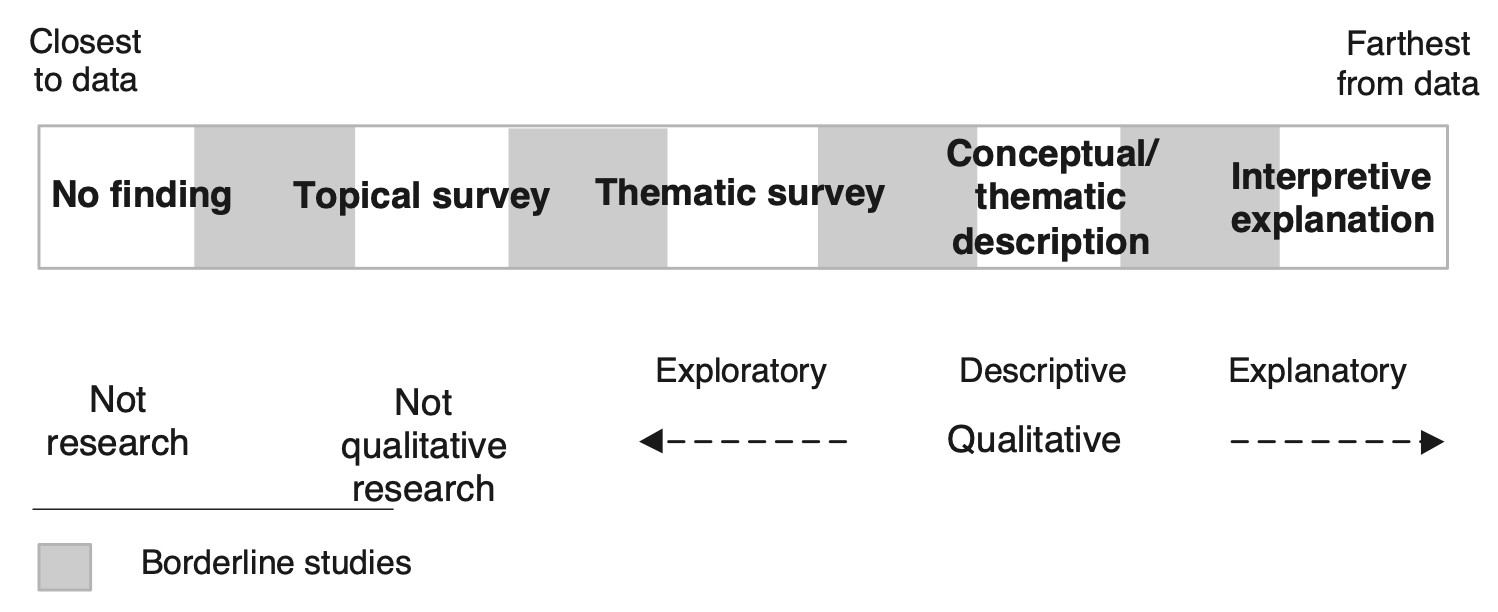
\includegraphics[width=1\linewidth]{Images/Methodology/TypologyOfQualitativeFindings.png}
    \caption{Typology of Qualitative Findings \citep{sandelowski2003classifying}}
    \label{fig:typology}
\end{figure}

With this in mind, for the thesis, the aim of my analysis was to be a descriptive process of the participants' experiences. In such a way, the aim of my analysis fits in the middle point of the qualitative 'poles' in Sandelowski and Barroso figure where while I'm not engaging in data transformation to develop a theory, nor is my analysis purely descriptive of the original data. \citep{kiger2020thematic} suggest that thematic analysis is a proven approach that works well for providing highly descriptive and conceptual findings in their results. As thematic analysis provides steps to organise the data through labels and themes, the process provides transformative approaches to understanding the meanings and experiences of the participants within the data. 

The thematic analysis approach I followed was in line with the instructions set out by \cite{braun_one_2020}. This process consists of seven steps: 1) preparing data through transcripts and additional data cleaning; 2) familiarising myself with the data while referring to the research questions. Following, using a whiteboard / Miroboard - order the data to make sense of the similar conversations between participants; 3) move onto the coding process to identify all relevant data by line-by-line coding, tagging and highlighting anything of interest; 4) organise codes into potential linking themes; 5) reviewing themes; 6) discuss the initial themes with supervisors to see if they fit with the original research questions and name the themes. Finally, step 7) is to finalise the analysis by writing and presenting it in the data chapters. Data was collected and analysed chronologically to the chapters that are set out in the thesis.

\section{Reflexivity}
\label{Method:Reflectivity}
 As described in the following data chapter, the work I did within dementia significantly impacted my experiences of dementia within my family. I relate the comparisons and connections between my research and my conversations with my Grandma about my Grandpa's diagnosis. From early on, it was very apparent that my experiences during and outside the studies would influence the interpretations I made through my analysis. As such, Barbara Probst describes reflexivity as:
\begin{quote}
"Despite its "messiness," reflexivity remains a fundamental way, particularly in qualitative studies, to bolster credibility by parsing the research endeavor into its mutually affecting parts and documenting the pathways through which knowledge was generated." \citep{probst2015eye}
\end{quote}

Reflexivity offers a critical way to stay self-aware through the thesis. Still, more importantly, it is a way to acknowledge the emotional and often challenging experiences that a researcher may encounter when working within sensitive settings - like dementia. Throughout the PhD, I have made many relationships with participants I still talk to after finishing the study. For instance, Jim, a participant in my final study, will still email or occasionally Zoom to chat about dementia activist topics and general day-to-day conversations. This is often due to my early recruitment stages requiring openness from myself to get to know the participant and make them feel comfortable in my presence. Typically, participants would often ask my \textit{\textbf{"why are you looking into dementia?"}}Looking back at my reflexive journal - that researchers recommend for during the research process and coding stages, I found this excerpt from  replying to the question above:

\begin{quote}
    
\textbf{James}: Well, I'm not sure if you remember, but last year [2017] I worked with a couple of you to create some VR experiences that looked at ways to personalise the environments for members here [ at Silverline]. As I got to know the area more, I talked to my Grandma about my research. One of the reasons I thought about dementia research was because of her. My Grandpa had Alzheimer's in his early 50's. He sadly passed away when I was five… Of course, I didn't get to know him that well, but through the circumstances my Grandma shares stories of him. She shared stories of before the diagnosis and many that of her relationship with him after his diagnosis too.

\textbf{Kate}: "are you close with your Grandma?"

\textbf{James}: "Very much so... I call her every few days and we talk about all sorts… To me, It's been interesting to hear my Grandma's side towards caring for my Grandpa too. The stories of her having to learn how to organise the bills, or mortgage – she had to take on so many social roles that he once proudly had… But also, she told me when she told him to get off his back-side and stop feeling sorry for himself… She would make alternations around the house to ensure he could do many of the roles he once felt like he lost – at least to the extent that he thought he could see fit. 
\end{quote}

\textbf{My reflexive journal comment: 
}
\begin{quote}
"As I began to share stories of my family, Kate started to cry. Kate shared how much the story reflected her experiences too. We started to share stories from each family side. Kate had gone through similarities to my Grandma with having to change significant social and, even in their eyes, gender roles. I feel perhaps Kate and I have bonded over these stories. Maybe she trusts me more now she knows why I care for making some change in dementia? We both cried, laughed and smiled, listening to each other's stories. It felt strange to me that this felt so wrong. A relatively common interaction among friends, maybe not so much between somewhat strangers, but what made me feel 'wrong' was that my openness made me assume I was a bad researcher."
\end{quote}

Although the reflective texts in my journal are not part of the data I analysed, they helped with the personal development of my role as a researcher and to deal with some of the difficult conversations and topics that were present in conversations I had with people with dementia. Some of the more difficult conversations I had, I was fortunate to share with the cohort I started the PhD with. The way the Digital Civics PhD programme was designed gave many of us who had similar difficult conversations in other sensitive settings the chance to share and reflect on the processes of being a researcher together. Finally, by taking a reflective approach throughout the data collection and analysis, has provided I have examined the growing relationships that I have made through the study, my positioning in the dementia context, and understanding how I fit into the research and the responsibilities that come with the role of a researcher. 
\section{Summary}
\label{Method:summary}